% This LaTeX was auto-generated from MATLAB code.
% To make changes, update the MATLAB code and export to LaTeX again.

\documentclass{article}

\usepackage[utf8]{inputenc}
\usepackage[T1]{fontenc}
\usepackage{lmodern}
\usepackage{graphicx}
\usepackage{color}
\usepackage{listings}
\usepackage{hyperref}
\usepackage{amsmath}
\usepackage{amsfonts}
\usepackage{epstopdf}
\usepackage{matlab}

\sloppy
\epstopdfsetup{outdir=./}
\graphicspath{ {./ejercicio07_images/} }

\matlabmultipletitles

\begin{document}

\matlabtitle{Ejercicio Nº7}


\begin{matlabcode}
clear;clc;
\end{matlabcode}

\vspace{1em}

\begin{matlabcode}
syms t vc1(t) vc2(t) il1(t) il2(t);
\end{matlabcode}

\matlabheading{Valores de los componentes}

\begin{matlabcode}
g1=1;
g2=2;
g3=3;
g4=4;
L1=1;
L2=1;
C1=1;
C2=1;
\end{matlabcode}

\begin{par}
\begin{flushleft}
Se plantean las ecuaciones y se obtienen las matrices de la forma generalizada
\end{flushleft}
\end{par}

\begin{matlabcode}
M=[C1*(1/g1 + 1/g3) 0 0 0;0 0 L1 -L2;-C1/g3 C2/g4 0 L2;0 C2*(-1/g2-1/g4) 0 0];
N=[1 0 1/g1 -1/g3;-1 1 0 0;0 0 0 1/g4+1/g3; 0 -1 1/g2 -1/g4];
u=[0;0;0;0];

\end{matlabcode}

\begin{par}
\begin{flushleft}
Se expresan las matrices de la forma normalizada
\end{flushleft}
\end{par}

\begin{matlabcode}
A=-1.*(M\N)
\end{matlabcode}
\begin{matlaboutput}
A = 4x4    
   -0.7500         0   -0.7500    0.2500
         0   -1.3333    0.6667   -0.3333
    0.7500   -0.6667   -0.4167   -0.4167
   -0.2500    0.3333   -0.4167   -0.4167

\end{matlaboutput}
\begin{matlabcode}
B=M\u
\end{matlabcode}
\begin{matlaboutput}
B = 4x1    
     0
     0
     0
     0

\end{matlaboutput}
\begin{matlabcode}
vc01=1;
vc02=0;
il01=0;
il02=0;
Xant=[vc01;vc02;il01;il02]
\end{matlabcode}
\begin{matlaboutput}
Xant = 4x1    
     1
     0
     0
     0

\end{matlaboutput}
\begin{matlabcode}
[T, lambda] = eig(A);
syms t;
elambda=diag(exp(eig(A).*t));
vpa(elambda,4)
\end{matlabcode}
\begin{matlabsymbolicoutput}
ans = 
    $\displaystyle \left(\begin{array}{cccc}
e^{t {\left(-0.5563+0.9145 i\right)}}  & 0 & 0 & 0\\
0 & e^{t {\left(-0.5563-0.9145 i\right)}}  & 0 & 0\\
0 & 0 & e^{-1.125 t}  & 0\\
0 & 0 & 0 & e^{-0.6786 t} 
\end{array}\right)$
\end{matlabsymbolicoutput}
\begin{matlabcode}
H=T*elambda*inv(T);
v=H*Xant;
\end{matlabcode}


\begin{par}
\begin{flushleft}
Expresando la tensión vg4 en función de las corrientes IL2 e IC2
\end{flushleft}
\end{par}

\begin{matlabcode}
Ic2=C2*diff(v(2,:),t);
Vg4=(v(4,:)+Ic2)/g4;
vpa(Vg4,4)
\end{matlabcode}
\begin{matlabsymbolicoutput}
ans = 
    $\displaystyle e^{-1.125 t}  {\left(-0.1434+1.625 {10}^{-17}  i\right)}+e^{-0.6786 t}  {\left(-0.07908+1.431 {10}^{-17}  i\right)}+e^{t {\left(-0.5563-0.9145 i\right)}}  {\left(0.1112-0.004343 i\right)}+e^{t {\left(-0.5563+0.9145 i\right)}}  {\left(0.1112+0.004343 i\right)}$
\end{matlabsymbolicoutput}


\matlabtitle{Trayectorias de estado}

\begin{matlabcode}
%Valores de los componentes
g1=1;g2=2;g3=3;g4=4;L1=1;L2=1;C1=1;C2=1;
%Condiciones Iniciales
vc1=1;vc2=0;il1=0;il2=0;

%Valores de tiempo y paso
ti=0;tf=10;
h=0.01;

%Matrices del circuito 
%Lleva la forma de:
%M*(dx/dt)+N*x=u(t);

M=[C1*(1/g1 + 1/g3) 0 0 0;0 0 L1 -L2;-C1/g3 C2/g4 0 L2;0 C2*(-1/g2-1/g4) 0 0];
N=[1 0 1/g1 -1/g3;-1 1 0 0;0 0 0 1/g4+1/g3; 0 -1 1/g2 -1/g4];
u=[0;0;0;0];

%Condiciones iniciales
Xant=[vc1;vc2;il1;il2];

%Se lleva a la forma 
% dx/dt=q(t)-P*x

P=-1.*(M\N);
solu=[];
%Método RK4
it=1;
for i= ti:h:tf
    k1= (q+P*Xant).*h;
    Xant2=Xant+(k1.*0.5);
    k2=(q+P*Xant2).*h;
    Xant3=Xant+(k2.*0.5);
    k3=(q+P*Xant3).*h;
    Xant4=Xant+k3;
    k4=(q+P*Xant4).*h;
    X=Xant+(k1+2.*k2+2.*k3+k4)/6;
    solu=[solu X];
    Xant=X;
    it=it+1;
end
solu=solu';
t=ti:h:tf;
\end{matlabcode}


\begin{matlabcode}
plot(solu(:,3),solu(:,1),'-b');
hold on 
plot(solu(:,3),solu(:,2),'-g');
hold on 
plot(solu(:,4),solu(:,1),'-r');
hold on 
plot(solu(:,4),solu(:,2),'-m');
hold off
title('Phase portrait');
xlabel('Corriente');
ylabel('Tensión'); 
legend({'VC1 vs iL1','VC2 vs iL1','VC1 vs iL2','VC2 vs iL2'})
\end{matlabcode}
\begin{center}
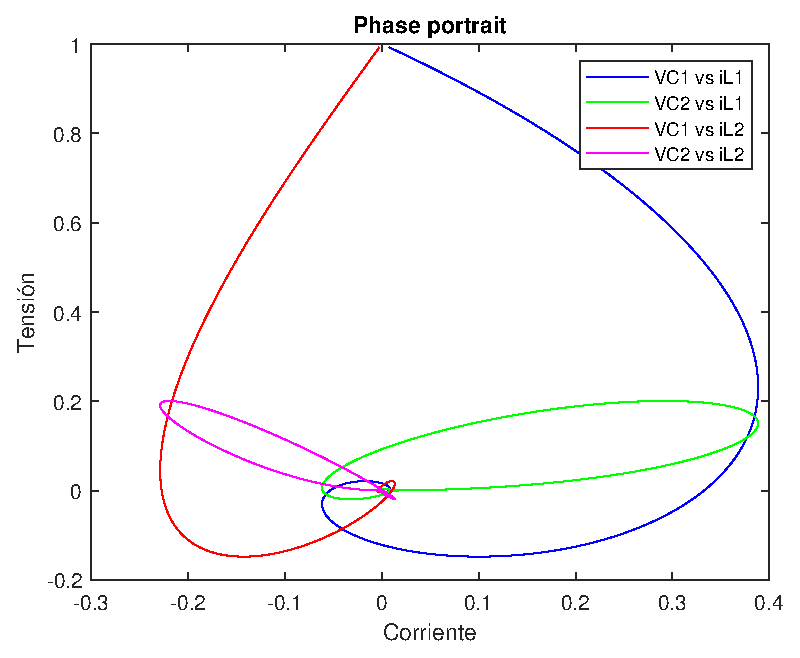
\includegraphics[width=\maxwidth{56.196688409433015em}]{figure_0_07}
\end{center}

\end{document}
